\documentclass[letter,12pt]{article}


\usepackage{lineno}
\usepackage{setspace}
\usepackage{graphicx}
\usepackage{subfigure}
\usepackage{float}
\usepackage{color}
\usepackage{caption}
\usepackage[margin=1in]{geometry}
\usepackage{epstopdf}


\begin{document}
\doublespacing
\linenumbers



\noindent RH: LANDERER ET AL.--- Intragenomic variation in codon usage
% put in your own RH (running head)
% for POVs the RH is always POINT OF VIEW
i
\bigskip
\medskip
\begin{center}

% Insert your title:
\noindent{\Large \bf Differences in Codon Usage Bias between genomic regions in the yeast \textit{Lachancea kluyveri}.}
\bigskip

% We don't use a special title page; the author information is entered
% like any other text.

% FOOTNOTES: We don't allow them in the manuscript, except in
% tables. Don't include any footnotes in the text.


\noindent{C\textsc{EDRIC} ~{L\textsc{ANDERER}}$^{1,2,*}$,
R\textsc{USSELL} {Z\textsc{ARETZKI}}$^{3}$,
\textsc{AND}
M\textsc{ICHAEL} A.~{G\textsc{ILCHRIST}}$^{1,2}$}

\end{center}

\vfill

{\small
\noindent$^{1}$Department of Ecology \& Evolutionary Biology, University of Tennessee, Knoxville, TN 37996-1610\\
\noindent$^{2}$National Institute for Mathematical and Biological Synthesis, Knoxville, TN 37996-3410\\
\noindent$^{3}$Department of Business Analytics \& Statistics, Knoxville, TN ~ 37996-0532 \\
\noindent$^{*}$Corresponding author. E-mail:~cedric.landerer@gmail.com
}

\vfill
\centerline{Version dated: \today}
\vfill
\newpage

\begin{abstract}
Codon usage bias (CUB), the differential non-uniform usage of synonymous codons, can vary greatly between genes within an organism and across organisms due to mutation bias or selective constrains. 
Large efforts have been made to develope and explore models to understand intra-genomic variation in codon usage and the contributions of mutation and selection to its evolution.
Comparative studies have been undertaken to further our understanding of variation in codon usage between species.
However, limited efforts have been made to understand how CUB is affected, and in return affects hybridization or introgression events between species with potentially large differences in CUB. 
In this study, we explore the signature of CUB of \textit{Lachancea kluyveri}, a yeast that has experienced a large introgression covering the whole left arm of chromosome C and about 10\% of all genes.
The introgression event found in the \textit{L. kluyveri} genome make this yeast an ideal candidate to explore intra and inter-genomic differences in CUB.
The \textit{L. kluyveri} genome provides insights about the adaptation of introgressed regions to the novel genomic host environment, with potentially large differences in selection due to shifts in selective constraints like tRNA availability, the effectiveness of selection due to a change in effective population size, or differences in mutation bias.
We analyzed patterns of codon usage across the \textit{L. kluyveri} genome and separated the effects of mutation bias and selection for translation efficiency on CUB.
The results were compared to the effects of mutation and the strength of selection in the native genome and the introgressed region. 
Our results show distinct patterns of CUB between the introgressed region C-Left and the remaining \textit{L. kluyveri} genome.
In addition we were able to determine that the difference in CUB is mostly driven by differences in mutation bias between C-Left and the remaining genome.
The introgression in the \textit{L. kluyveri} genome is of additional interest as the source organism has not yet been identified.
Given our ability to clearly distinguish codon usage between the introgressed region and the \textit{L. kluyveri} genome we  further explored if CUB is suitable to identify possible candidates for the origin of the introgressed region C-Left.
The estimation of CUB across a variety of yeast species allowed us to identify candidates for the origin of C-Left.
We validated the candidates identified using CUB by comparing GC-content and synteny relationships between C-Left and the candidates.
\end{abstract}


\section*{Introduction}

Organisms undergo changes in phenotype due to selection on fitness relevant traits in their current environment. 
The same principle applies to the genome adapting to the intra-cellular environment.
If genomes are mixed, due to hypridization or introgression events, the part of the genome new to the current intra-cellular environment experiences added selection pressure to adapt to the new environment.

\textit{Lachancea kluyveri} is the earliest diverging lineage of the known \textit{Lachancea} clade and diverged from the \textit{Saccharomyces} lineage prior to the whole-genome duplication 100 Ma ago (Wolfe and Shields 1997). 
However, \textit{L. Kluyveri} and \textit{S. cerevisiae} share a similar life cycle.
\textit{L. Kluyveri} experienced an introgression of 1Mb about XXX ago. 
The introgression shows a difference in average GC-content of \~ 13 \% compared to the rest of the \textit{L. Kluyveri}.

Patterns of genomic variation help understanding evolution, but are mostly explored between and within species and populations.
Intra-genomic variation due to differential mutation, selection or hybridization is often ignored.
The analysis differences in patterns of codon usage allows us to explore differential evolution within a genome and differentiate between the effects of mutation and selection.

We asked if the difference in GC-content is reflected in differences in codon usage bias.
We analyzed the two genomic regions in the \textit{L. Kluyveri} genome together and separately.
Our results indicate that the introgressed region shows a different signature of codon usage bias.
We employed a mechanistic model that allowed us to distinguish between effects of mutation bias, or bias in selection for translation efficiency.
Further inspection showed that mutation bias is dominating the observed difference, while differences in selection bias between codons is mostly in agreement between the two genomic regions. 

Various attempts have been made to explain why C-Left shows a strong difference in GC-Content.
Here, we analyze C-Left and explore signals of intra-genomic heterogeneity in mutation and selection between C-Left and the rest of the genome using signals of codon usage bias.
The differential usage of synonymous codons is shaped by differences in nucleotide stability, and selection for translation efficiency and error reduction.
Nucleotide stability varies, and introduces a mutation bias between synonymous codons, prevalent in low expression genes with weak selection for translation efficiency.
In contrast, selection for translation efficiency is strong in highly expressed genes, allowing for the estimation of differences in selection bias between synonymous codons.

Selection on codon usage is assumed to be associated with the available tRNA pool in a cell. 
Codons matching more abundant tRNA species are assumed to minimize ribosome pausing due to reduced waiting time for a correct tRNA. 
Differing codon usage bias in the introgressed region can either be caused by differences in mutation bias, or differences in selection for translation efficiency, indicate a shift in the available tRNA pool.
Differences in mutation bias should persist longer due to the absence of selection.   

	
\section{Materials \& Methods}

\subsection{Estimating codon usage bias}
We analyzed the coding genes of several yeast species (see Table \ref{org_overview}) using ROC-SEMPPER \cite{gilchrist2015} implemented in the R package AnaCoDa (Landerer et al. 2017).
In the case of \textit{L. kluyveri} we analyzed the codon usage pattern for the whole genome and separated C-Left from the rest of the genome for differential analysis of the codon usage patterns.
We compared the estimated codon parameters for mutation bias $\Delta M$ and selection bias $\Delta \eta$ for all yest species to the estimated $\Delta M$ and $\Delta \eta$ values of C-Left using Pearson correlation.
For \textit{L. kluyveri} we compared the two model fits for the whole genome and for the genome split using AIC as well as compared the estimated protein synthesis rates $\phi$ to observed gene expression data from XXX.

\subsection{Estimating phylogenetic tree and divergence time}
To estimate the divergence time between \textit{L. kluyveri} and C-Left, we appropriated a dataset of several yeast species from Salichos and Rokas (2013). 
We decided to drop \textit{S. bayanus} from the tree as it is the result of a hybridization between \textit{S. eubayanus} and \textit{S. cerevisiae}.
We re-estimated the species tree by concatenation of all CDS found on the \textit{L kluyveri} main genome using RAxML (Stamatakis 2014) on the CIPRES Gateway (Miller et al. 2010).
We repeated the same process using only genes found on C-Left of \textit{L kluyveri}.
The divergence time was estimated by determining the rate of evolution $\sigma^2$ of the $\Delta M$ parameters estimated for each yeast species.
We only utilized $\Delta M$ and not $\Delta \eta$ as these values are reflecting the strength of selection $s$ relative to the effective population size $N_e$ and therefore can not be assumed to evolve neutral.
As the variance under a brownian motion diffusion process growth with time at a constant rate $\sigma^2$, we can calculate the variance of the diffusion process at any given time $\sigma^2_t$. 
We solved $\sigma^2_t = t\sigma^2$ for $t$ to find the combined maximum likelihood estimate for $t$ for all 40 rate estimates.
The confidence intervals for $t$ was obtained from the profile likelihood by calculating where the likelihood function drops by two units.
  
\subsection{Determination of synteny}	
The complete genomes of several yeast species along the phylogeny were downloaded from the NCBI genome database.
Whole genome alignments where performed using SyMAP v4.2 (Soderlund et al. 2006, Soderlund et al. 2011).
We analyzed synteny relationships between C-Left and the genomes of several yeast species to understand where along the phylogenetic tree synteny breaks down.
  
	
\section*{Results}
The striking difference in GC-content between C-Left and the rest of the \textit{L. kluyveri} genome lead us to the question whether the observed differences in GC-content are an indicator for intra-genomic variation in codon usage bias.
We hypothesised that the observed GC-content variation in the \textit{L. kluyveri} genome and the codon usage bias are independent, and we will not observe intra-genomic variation in codon usage bias.
Analysis of the \textit{L. kluyveri} genome with ROC SEMPER revealed low variation in predicted protein synthesis rate $\phi$, indicating strong disagreement in genome wide parameters and hinting at intra-genomic variation.
  
To test whether C-Left shows distinguished codon usage patterns, we separated C-Left from the rest of the genome and analyzed both parts of the genome separately.
Separation of the genome was strongly favored by model selection ($\Delta AIC: 81,504$) indicating differing patterns of codon usage bias between C-Left and the rest of the genome.

\subsection*{\textit{L.kluyveri} displays differential codon usage bias}
The separation of the genome into two independent part improved our ability to predict protein production rate $\phi$ (H0: $\rho = 0.59$ to H1: $\rho = 0.69$).
Using the whole genome, $\phi$ almost perfectly separated the genes of C-Left and the rest of the \textit{L. kluyveri} genome. 
The separation resulted in genes that are not located on C-Left to be estimated to be medium to high expressed while genes located on C-Left were estimated to be low expression genes. 
This separation of C-Left from the rest of the genome resulted into low and high expression genes resulted in mutation bias ($\Delta M$) being only informed by genes on C-Left while selection for translation efficiency ($\Delta \eta$) being only informed by genes not located on C-Left. 
In addition, the standard deviation of the $\phi$ distribution of the whole genome was greatly decreased compared to the separated dataset (H0 : $s_{\phi}$ = 0.2 to H1 : $s_{\phi}$ = 1).

\subsection*{Differences in mutation bias are greater than in selection bias}
The hypothesis best supported by the data allows us to attribute differences in GC-content mostly to mutation bias. 
A greater difference in mutational bias between the two genomic regions is revealed while selection for translation is mostly consistent between the two genomic regions. 
The comparison of the estimated mutation bias ($\Delta M$) resulted in strong disagreement in codons being favored by mutation ($\rho = -0.31$). 
Most codons that show a positive mutation bias in C-left are disfavored by mutation in the remainder of the genome.  
Furthermore, the strength of mutation bias is increased in C-left, reflected in the larger range of inferred $\Delta M$ values, revealing not only differences in mutation bias, but also showing that mutation bias in C-Left is stronger than in the rest of the genome. 
Estimates for $\Delta \eta$ showed a higher consistency between the two genomic regions ($\rho = 0.68$), indicating that - generally - the same codons are favored throughout the genome. 
The difference in time scale of protein synthesis rate $\phi$ between C-Left and Main, does not allow to draw any conclusions from the observed differences in range of the inferred $\Delta \eta$ parameter.

\subsection*{Comparing codon usage of various yeast species}
We determined the codon usage patterns of 38 related yeast species to explore if one of the species shows a similar codon usage pattern.
Agreement in codon usage patterns between C-Left and other yeast species would hint at a possible origin of C-Left.
We found that codon usage is conserved across most of the here analyzed yeast. 
Most yeast displayed high agreement in codon usage with the main part of the \textit{L. kluyveri} genome. Of the 38 analyzed yeast, 26 show a correlation $\rho > 0.5$ for the selection bias term $\Delta \eta$ and 32 for the mutation bias term $\Delta M$.
However, when we compared the codon usage of C-Left to the other yeast, we found only four showing a correlation $\rho > 0.5$ for $\Delta M$ but 25 yeast for $\Delta \eta$ (Figure~\ref{fig:csp_cor_all_yeast}).
Of the four yeast species with high agreement in mutation bias only three (\textit{C. albicans}, \textit{C. dubliniensis}, and \textit{E. gossypii}) also showed high agreement in selection bias.

\subsection{GC content}
C-Left became of interest due to its remarkable difference in GC content compared to the rest of the \textit{L. kluyveri} genome.
\textit{L. kluyveri} shows a 13 \% increase in GC content strictly confined to C-Left. 
Previous work speculated that the origin of C-Left must be within the Lachancea clade since synteny can be found between C-Left, and \textit{L. thermotolerans} and \textit{L. waltii} (Payen et al 2009).
However, the Lachancea clade is not a monophyletic group.
The increased GC content in C-Left and the would therefore hint at a species closely related to \textit{L. kluyveri} with an elevated GC content. 
Our search identified only three closely related yeast with GC $> 50\%$ of which none is classified as a Lachancea (\textit{E. gossypii}, \textit{C. yegresii}, and \textit{S. musiva}).

\subsection*{Synteny between C-Left and other yeast genomes}

We evaluated genome synteny and rearrangements between several candidate genomes and \textit{L. kluyveri} C-Left using SynMap 4.2.
We were able to find further evidence of \textit{E. gossypii} as a potential origin for C-Left using genome synteny.
While synteny between \textit{L. kluyveri} and other Lachancea does occur, it is mostly limited to the main part of the genome.
Regions of synteny between C-Left and \textit{L. thermotolerans} and \textit{L. waltii} were previously reported (Payen et al. 2009) but disregarded as possible sources of origin due to their reduced GC content.

\subsection*{Rate of evolution of estimated parameters}
We used a phylogeny to estimate the rates at which $\Delta \eta$ and $\Delta M$ evolves in our set of taxa. 
We then treated C-Left as a new species and determined the divergence time between C-Left and the rest of the \textit{L. kluyveri} genome.
The divergence time was estimated using the 40 $\Delta M$ parameters estimated to estimate 40 rates under brownian motion. 
A divergence time of 0.96 (CI: 0.79-1.22) expected mutations was estimated as the maximum likelihood time over all 40 rate estimates.
We used this divergence time as branch length estimate to determine the minimum age of the C-Left introgression based on the observed codon usage pattern.
This allowed us to determine the height in the tree for a possible attachment of C-Left to the phylogenetic tree.

The length of the C-Left branch corresponded well with the divergence time between our previously determined candidate XXX. 
We only employed $\Delta M$ in the rate estimation as we can assume that mutation bias does evolve neutral.
We can not make this assumption for $\Delta \eta$ as it represents the strength of selection relative to the strength of drift ($sN_e$).

\section*{Discussion}

We analyzed the codon usage bias of \textit{L. kluyveri} and found differing codon usage between two previously identified distinct regions of the genome. 
The two genomic regions were analyzed in conjunction and separate for differences in mutation and selection bias underlying codon usage patterns.
Our findings indicate that C-Left shows great differences in mutations bias, and small differences in selection bias.
These findings have implications for the study of codon usage beyond the here studied \textit{L. kluyveri} as such studies assume common codon usage across the genome.
Even though the authors are not aware of other organisms with such remarkable introgression patterns, other sources such as strand bias can lead to differences in mutation bias.
Differences in mutation bias or even selection bias can distort or bias the results of codon usage analysis. 
As the comparison of experimental expression data to predicted protein synthesis rate $\phi$ shows, prediction of $\phi$ is still reasonable when ignoring differences in codon usage bias. 
However, we can not assume this to be always true and our prediction of $\phi$ is greatly improved when separating C-Left from the rest of the genome.
We also note that the variation in predicted $\phi$ is greatly reduced and most values are found around zero when the genome is not split.
This causes the model to reduce the impact of extreme values in the codon usage spectrum, in this case caused by the strong disagreement in mutation bias $\Delta M$.

The evolution of codon usage is driven by three forces of evolution: mutation, selection and drift.
The insertion of a genomic region into a new host environment is expected to lead to adaptation in the inserted region.
Neutral change is slow as no selection is amplifying the proliferation of introduced changes.
We therefore, expect that differences in mutation bias, driving codon usage in low expression genes, to decay slower than differences in selection bias.
C-Left shows an access number of genes with low evolutionary mean expression.
The slow decay of mutation bias is supported by an excess of polymorphisms of low frequency, like expected under a model of neutral evolution (Friedrich 2014).

Attempts to elude on the unknown history of C-Left have been plenty full.
Here, we used the opportunity to see if the analysis of codon usage bias can be used to help elude on this question.
Our comparison of codon usage patterns across various yeast species revealed three promising candidate as origin of C-Left.
The first two \textit{C. albicans} and \textit{C. dubliniensis} show very low GC content compared to C-Left with 34 \% and 33 \% respectively. 
Furthermore, neither shows any synteny relationship with C-Left.
Therefore, depsite the low estimated divergence time between C-Left and these organisms, we have to disregard them as potential donor organisms. 
The third organism \textit{E. gossypii} however shows similar codon usage, GC content (52 \%), and high synteny.  

\section{Acknowledgments}


%\bibliographystyle{plain}
\bibliography{kluyveri_ref}


\section{Figures and Tables}

\begin{table}
\begin{tabular}{ | l | c | c | c | c | c | }
\hline
	Species & Timetree(mean) & Timetree(median) & Tree  & CUB(Main) & CUB(C-Left) \\ \hline
	Klac & 104 & 102 & 1.43 & 0.24 & 1.05 \\ \hline
	Agos & 104 & 102 & 1.43 & 1.53 & 1.62 \\ \hline
	Kthe & 85.7 & 85.7 & 1.39 & 0.46 & 1.08 \\ \hline
	Kwal & 85.7 & 85.7 & 1.39 & 0.43 & 1.04 \\ \hline
	Zrou & 114 & 112 & 1.48 & 0.25 & 1.11 \\ \hline
	Kpol & 114 & 112 & 1.48 & 0.4 & 1.28 \\ \hline
	Cgla & 114 & 112 & 1.48 & 0.4 & 1.18 \\ \hline
	Scas & 114 & 112 & 1.48 & 0.37 & 1.14 \\ \hline
	Skud & 114 & 112 & 1.48 & 0.2 & 1.01 \\ \hline
	Smik & 114 & 112 & 1.48 & 0.26 & 1.1 \\ \hline
	Spar & 114 & 112 & 1.48 & 0.28 & 1.09 \\ \hline
	Scer & 114 & 112 & 1.48 & 0.17 & 1.05 \\ \hline
	Psti & 304 & 239 & 1.63 & 0.35 & 1 \\ \hline
	Cgui & 304 & 239 & 1.63 & 0.5 & 1.04 \\ \hline
	Clus & 304 & 239 & 1.63 & 0.64 & 1.45 \\ \hline
	Dhan & 304 & 239 & 1.63 & 0.32 & 1.11 \\ \hline
	Ctro & 304 & 239 & 1.63 & 0.72 & 1.45 \\ \hline
	Calb & 304 & 239 & 1.63 & 0.87 & 0.78 \\ \hline
	Cdub & 304 & 239 & 1.63 & 1.01 & 0.82 \\ \hline
	Cpar & 304 & 239 & 1.63 & 0.65 & 1.17 \\ \hline
	Lelo & 304 & 239 & 1.63 & 0.44 & 1.06 \\ \hline
\end{tabular}
\caption{}
\label{tab:div_time}
\end{table}


\begin{table}
\begin{tabular}{ | l | l | l | c | l | l | }
\hline
	Taxon 				& Abbreviation 	& NCBI taxonomic ID 	& \% GC & GC Source  		& CDS Source \\ \hline
	Candida albicans 		& Calb 		& 5476 			& 34 	& NCBI Genome DB 	& KEGG \\ \hline
	Saccharomyces bayanus 		& Sbay 		& 4931 			& 40 	& NCBI Genome DB 	& yeastgenome \\ \hline
	Trichophyton benhamiae 		& Tben		& 63400 		& 49 	& NCBI Genome DB 	& KEGG \\ \hline
	Tetrapisispora blattae 		& Tbla 		& 1071379 		& 32 	& NCBI Genome DB 	& KEGG \\ \hline
	Saccharomyces castellii 	& Scas 		& 27288 		& 37 	& NCBI Genome DB 	& yeastgenome \\ \hline
	Saccharomyces cerevisiae 	& Scer 		& 4932 			& 38 	& NCBI Genome DB 	& yeastgenome \\ \hline
	Eremothecium cymbalariae 	& Ecym 		& 45285 		& 40 	& NCBI Genome DB 	& KEGG \\ \hline
	Torulaspora delbrueckii 	& Tdel 		& 4950 			& 42 	& NCBI Genome DB 	& KEGG \\ \hline
	Candida dubliniensis 		& Cdub 		& 42374 		& 33 	& NCBI Genome DB 	& KEGG \\ \hline
	Lodderomyces elongisporus 	& Lelo 		& 36914 		& 37 	& NCBI Genome DB 	& KEGG \\ \hline
	Saccharomyces eubayanus 	& Seub 		& 1080349 		& 40 	& NCBI Genome DB 	& ENA \\ \hline
	Debaryomyces fabryi 		& Dfab 		& 58627 		& 36 	& NCBI Genome DB 	& ENA \\ \hline
	Candida glabrata 		& Cgla 		& 5478 			& 39 	& NCBI Genome DB 	& KEGG \\ \hline
	Meyerozyma guilliermondii 	& Mgui 		& 4929 			& 44 	& NCBI Genome DB 	& KEGG \\ \hline
	Debaryomyces hansenii 		& Dhan 		& 4959 			& 36 	& NCBI Genome DB 	& KEGG \\ \hline
	Lachancea kluyveri 		& Lku 		& 4934 			& 40/53 & Payen et al. 2009 	& yeastgenome \\ \hline
	Saccharomyces kudriavzevii 	& Skud 		& 114524 		& 41 	& NCBI Genome DB 	& yeastgenome \\ \hline
	Kluyveromyces lactis 		& Klac 		& 28985 		& 39 	& NCBI Genome DB 	& KEGG \\ \hline
	Lachancea lanzarotensis 	& Llan 		& 1245769 		& 44 	& NCBI Genome DB 	& ENA \\ \hline
	Yarrowia lipolytica 		& Ylip 		& 4952 			& 49 	& NCBI Genome DB 	& KEGG \\ \hline
	Clavispora lusitaniae 		& Clus 		& 36911 		& 45 	& NCBI Genome DB 	& ENA \\ \hline
	Kluyveromyces marxianus 	& Kmar 		& 4911 			& 40 	& NCBI Genome DB 	& ENA \\ \hline
	Saccharomyces mikatae 		& Smik 		& 114525 		& 38 	& NCBI Genome DB 	& yeastgenome \\ \hline
	Sphaerulina musiva 		& Smus 		& 85929 		& 51 	& NCBI Genome DB 	& ENA \\ \hline
	Kazachstania naganishii 	& Knag 		& 588726 		& 46 	& NCBI Genome DB 	& ENA \\ \hline
	Saccharomyces paradoxus 	& Spar 		& 27291 		& 38 	& NCBI Genome DB 	& yeastgenome \\ \hline
	Candida parapsilosis 		& Cpar 		& 5480 			& 38 	& NCBI Genome DB 	& ENA \\ \hline
	Spathaspora passalidarum 	& Spas 		& 340170 		& 38 	& NCBI Genome DB 	& KEGG \\ \hline
	Tetrapisispora phaffii 		& Tpha 		& 113608 		& 34 	& NCBI Genome DB 	& KEGG \\ \hline
	Vanderwaltozyma polyspora 	& Vpol 		& 36033 		& 33 	& NCBI Genome DB 	& KEGG \\ \hline
	Lachancea quebecensis 		& Lque 		& 1654605 		& 47 	& Freel et al. 2016 	& ENA \\ \hline
	Zygosaccharomyces rouxii 	& Zrou 		& 4956 			& 40 	& NCBI Genome DB 	& KEGG \\ \hline
	Scheffersomyces stipitis 	& Ssti 		& 4924 			& 41 	& NCBI Genome DB 	& KEGG \\ \hline
	Lachancea thermotolerans 	& Lthe 		& 381046 		& 47 	& NCBI Genome DB 	& Genbank \\ \hline
	Candida tropicalis 		& Ctro 		& 5482 			& 33 	& NCBI Genome DB 	& KEGG \\ \hline
	Lachancea waltii 		& Lwal 		& 4914 			& 44 	& NCBI Genome DB 	& \  \\ \hline
	Cladophialophora yegresii 	& Cyeg 		& 470704 		& 54 	& NCBI Genome DB 	& ENA \\ \hline
	Eremothecium gossypii 		& Egos 		& 33169 		& 52 	& NCBI Genome DB 	& KEGG \\ \hline
\end{tabular}
\caption{}
\label{tab:org_overview}
\end{table}


\begin{figure}[H]
    \centering
    \begin{subfigure}
        \centering
        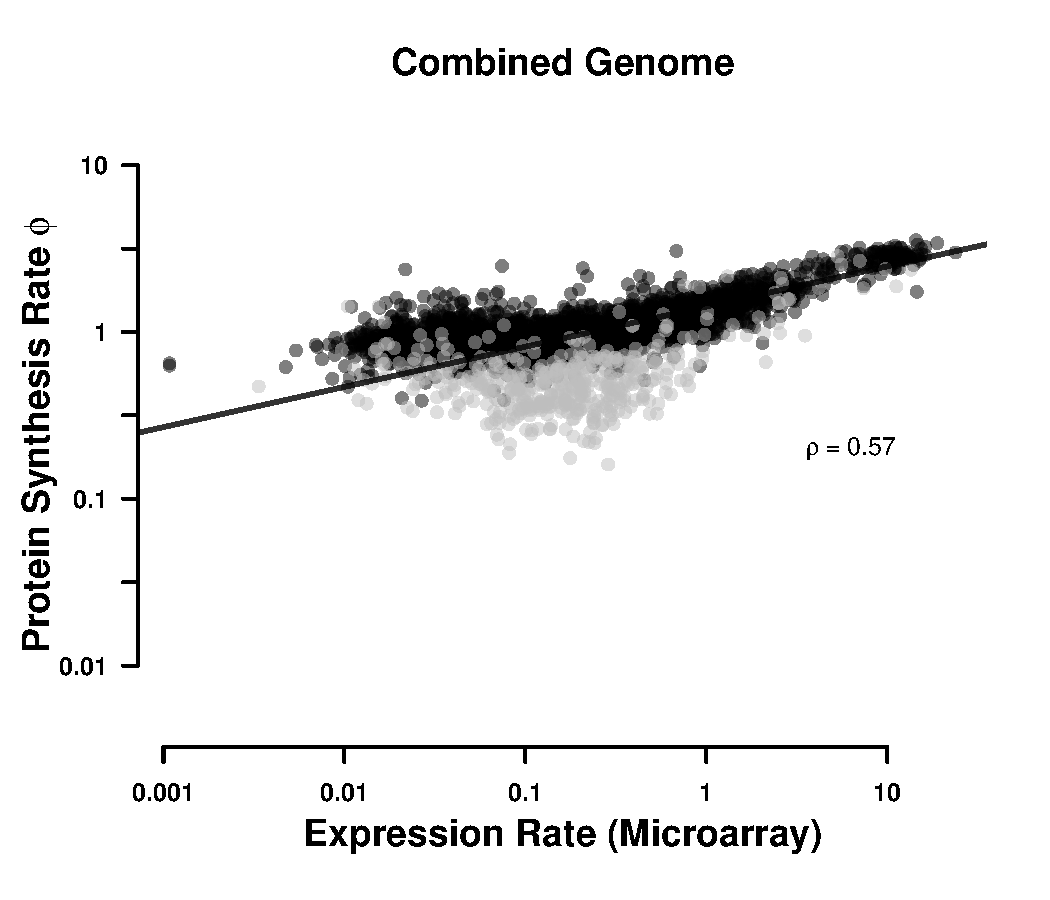
\includegraphics[width=.45\textwidth]{img/phi_corr_plot_whole_Genome_estim.pdf}
    \end{subfigure}
    \begin{subfigure}
        \centering
        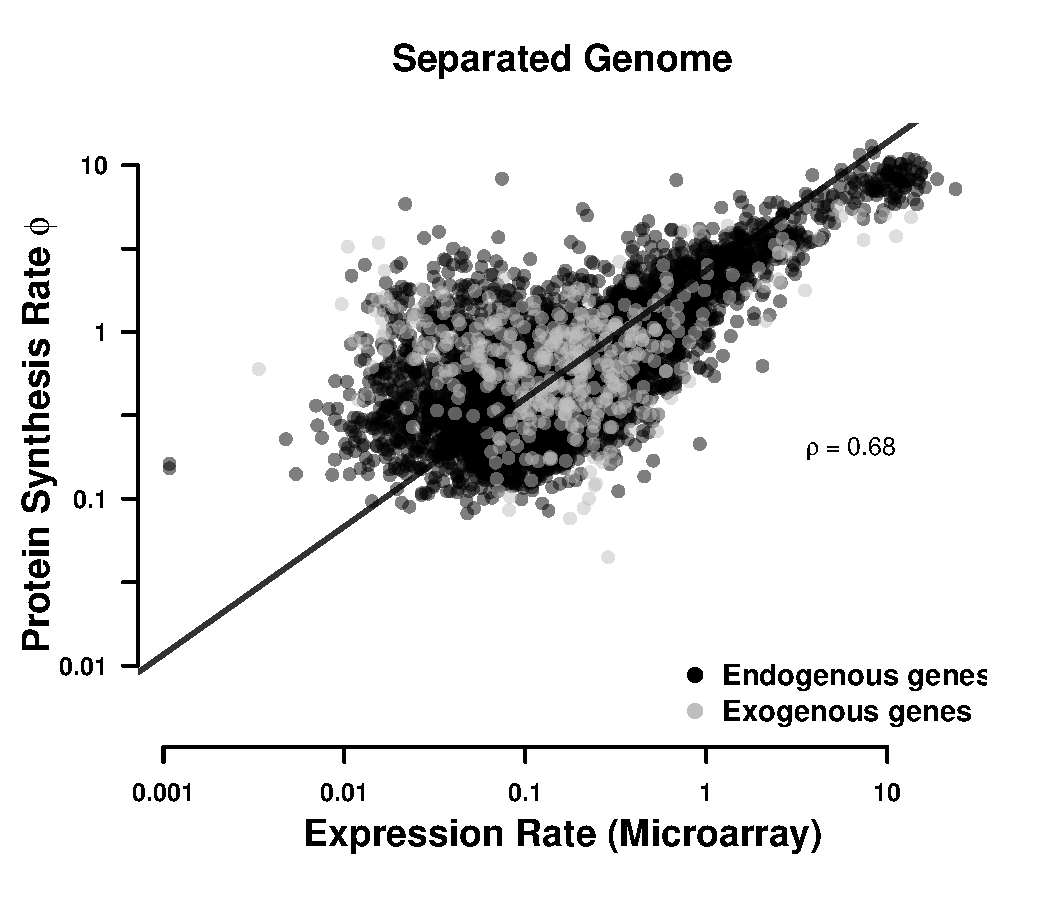
\includegraphics[width=.45\textwidth]{img/phi_corr_plot_split_Genome_estim.pdf}
    \end{subfigure}
    \caption{Person correltation of predicted protein synthesis rate $\phi$ with observed expression rate. )}
    \label{fig:phi_corr_two_cond}
\end{figure}

	
\begin{figure}[H]
    \centering
    \begin{subfigure}
        \centering
        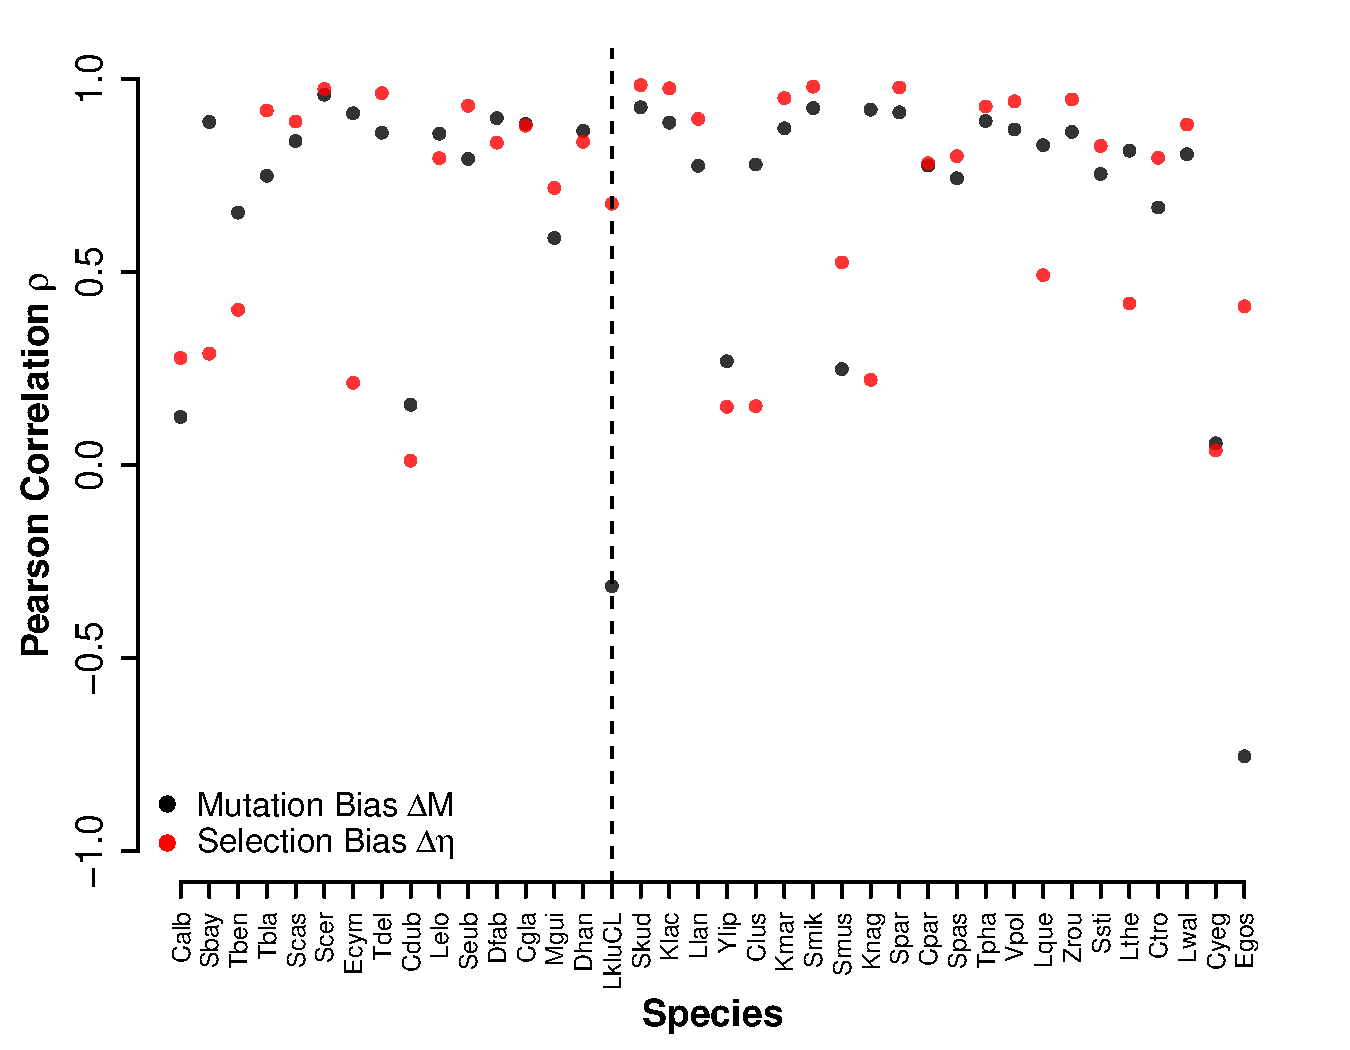
\includegraphics[width=.45\textwidth]{img/csp_all_species_vs_kuyveri_main.pdf}
    \end{subfigure}
    \begin{subfigure}
        \centering
        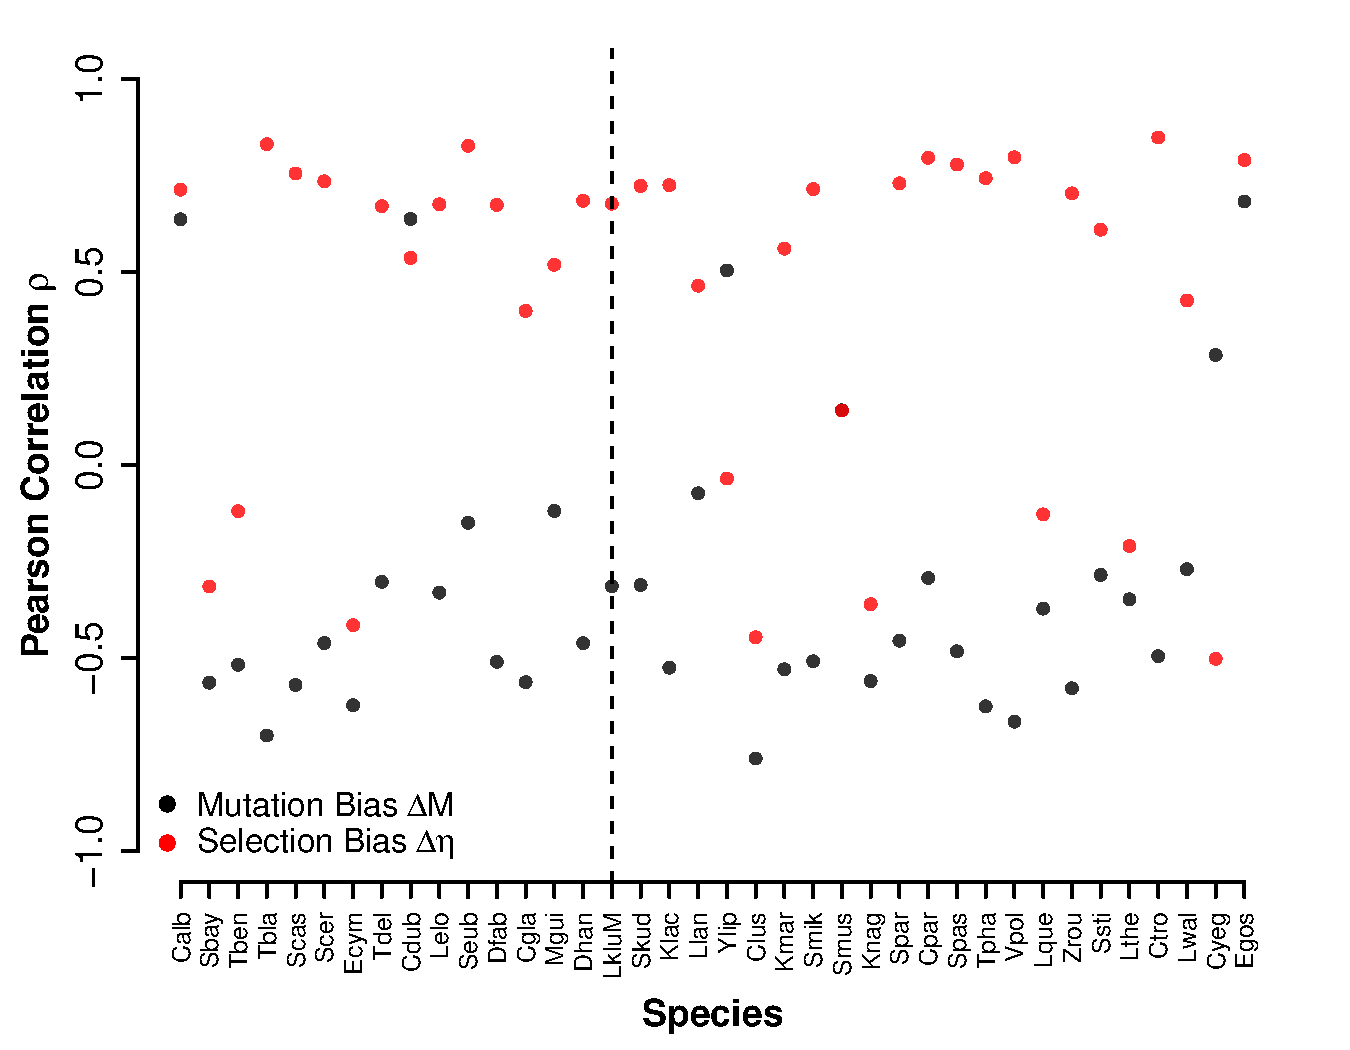
\includegraphics[width=.45\textwidth]{img/csp_all_species_vs_kuyveri_cleft.pdf}
    \end{subfigure}
    \caption{Person correlation of $\Delta \eta$ and $\Delta M$ of various yeast species with \textit{L. kluyveri} Main (a) and \textit{L. kluyveri} C-Left (b).}
    \label{fig:csp_cor_all_yeast}
\end{figure}

\begin{figure}[H]
    \centering
	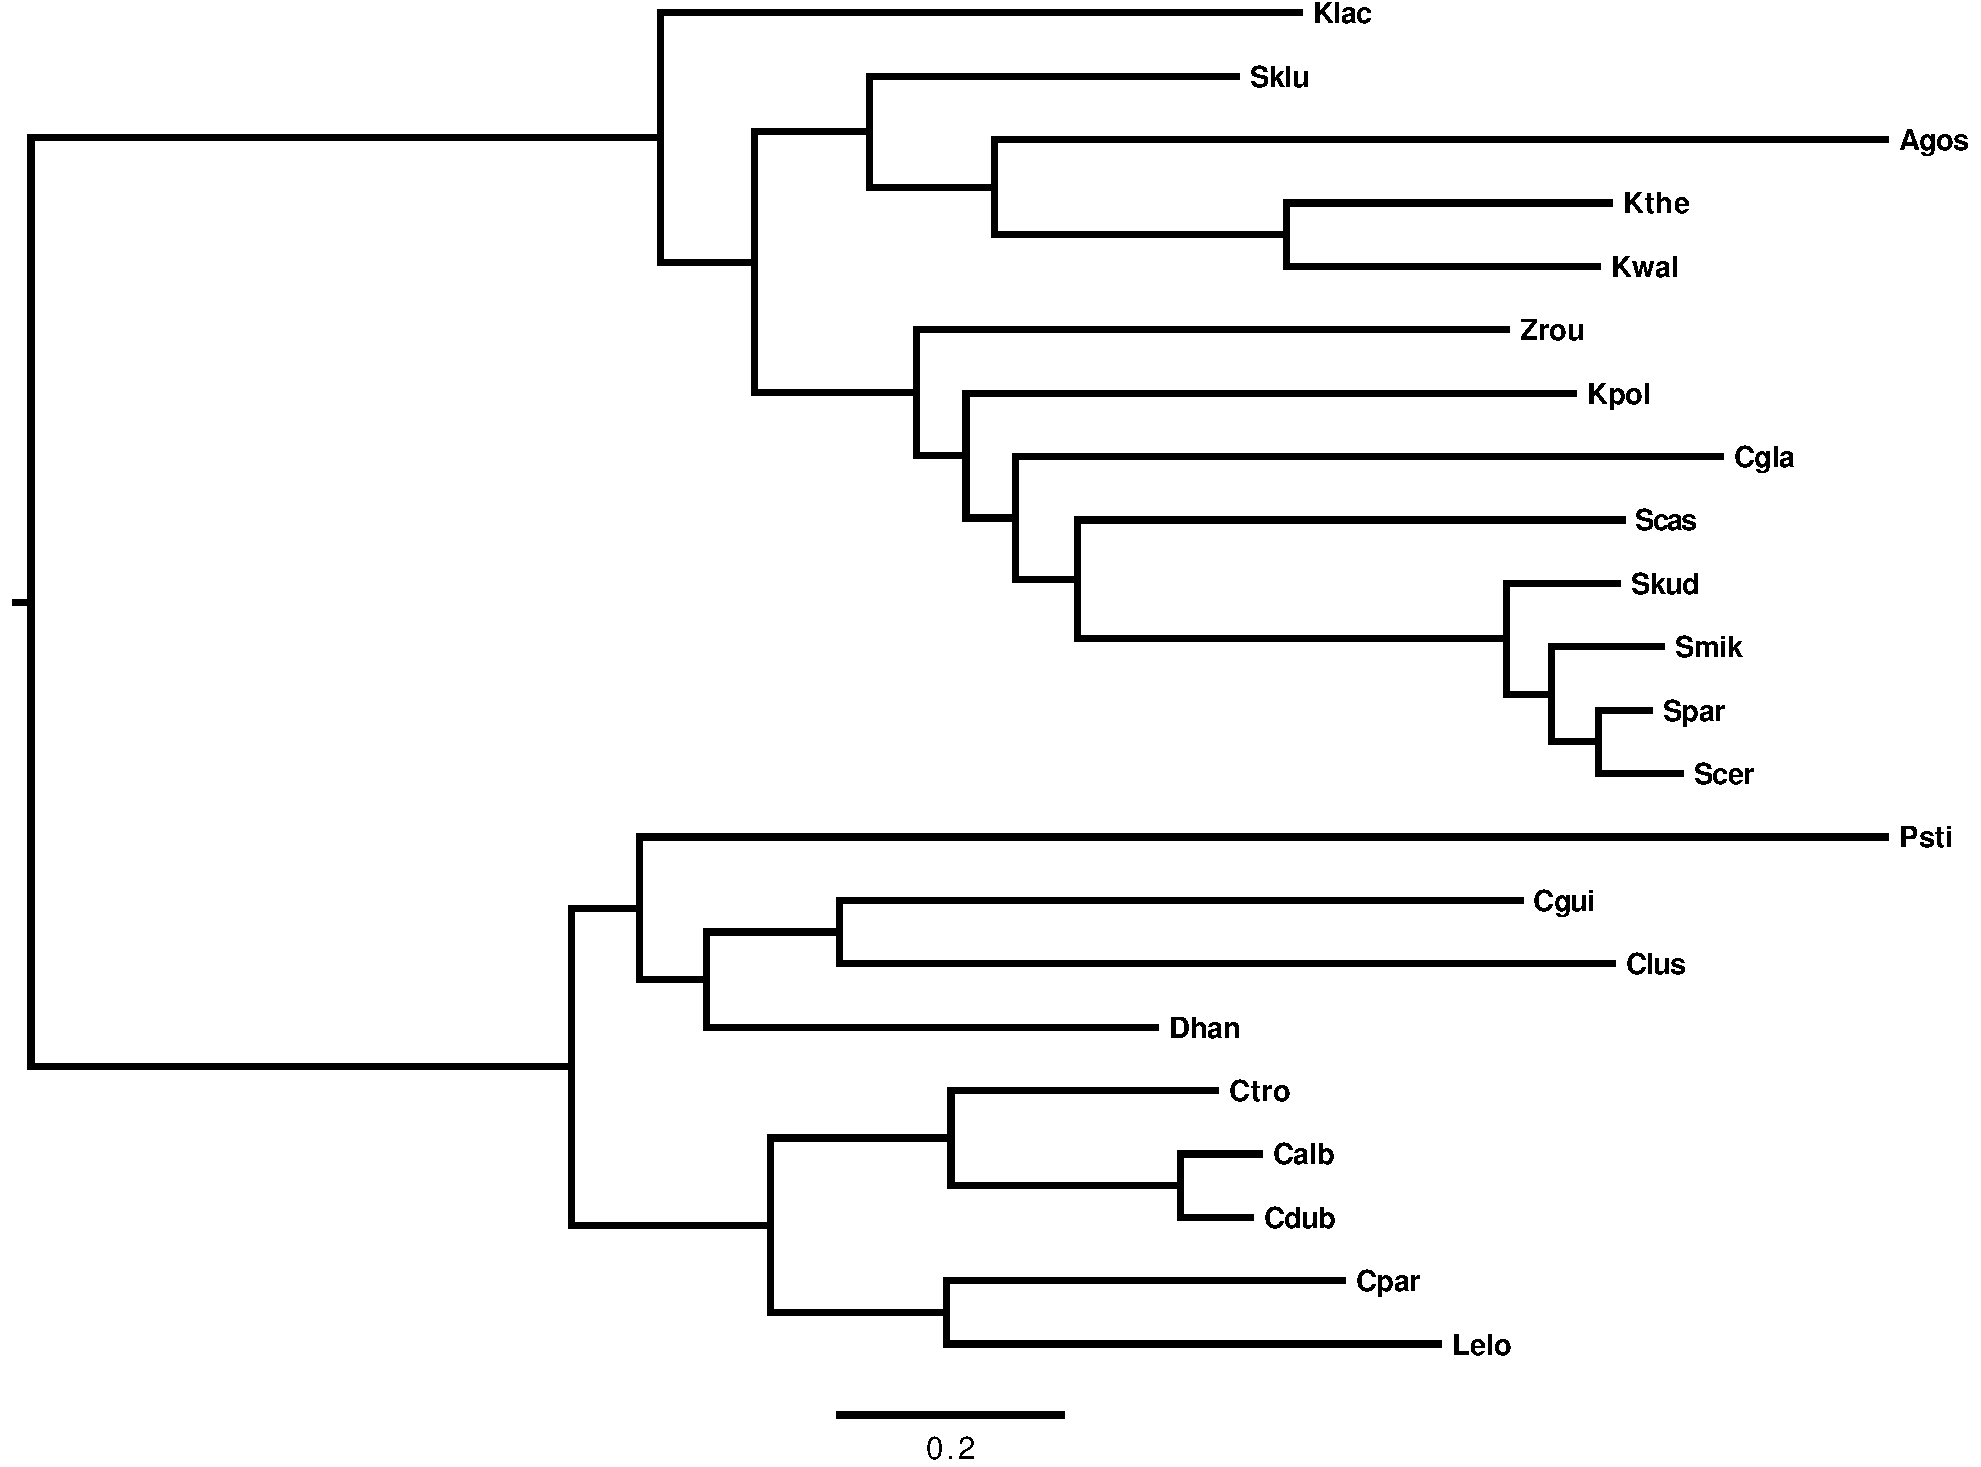
\includegraphics[width=0.8\textwidth]{img/rokas_noBay_RAxML_bestTree_rooted.pdf}
    \caption{}
    \label{fig:tree_yeast}
\end{figure}
\end{document}
